\documentclass[12pt]{amsart}
\usepackage{amsmath,amssymb,amsthm}
\usepackage{tikz}
\usetikzlibrary{arrows.meta,positioning,shapes.geometric}
\usepackage{xurl}
\usepackage[margin=1in]{geometry}

\newtheorem{lemma}{Lemma}[section]
\newtheorem{theorem}[lemma]{Theorem}
\newtheorem{corollary}[lemma]{Corollary}
\theoremstyle{definition}
\newtheorem{problem}[lemma]{Problem}

\newcommand{\NN}{\mathbb{N}}
\newcommand{\ZZ}{\mathbb{Z}}
\DeclareMathOperator{\sig}{\sigma}

\title{The Smallest Solution of $\sigma(an+1) > \sigma(an)$\\
for $a = 30$, $42$, and $70$}
\author{K. Subwattanachai}
\thanks{Department of Mathematics, Kasetsart University, Bangkok, Thailand}
\date{\today}

\begin{document}

\begin{abstract}
Pongsriiam (2024) asked for the smallest positive integer $n$ satisfying
$\sigma(an+1) > \sigma(an)$ for several small squarefree moduli $a$.
We adapt Martin's (1999) method for Euler's totient to the sum-of-divisors
function and compute the smallest $n$ for $a = 30$, $42$, and $70$.
The results are $n_{30} \approx 1.30 \times 10^{64}$ (65~digits),
$n_{42} \approx 6.69 \times 10^{41}$ (42~digits), and
$n_{70} = 48\,049\,097$ (8~digits).
The enormous spread in size comes from a single factor: whether the modulus
blocks every small prime or leaves a ``gap prime'' available for building
a highly abundant $an+1$.
\end{abstract}

\maketitle

%=====================================================================
\section{Introduction}
%=====================================================================

For an integer $m \ge 1$, let $\sigma(m) = \sum_{d \mid m} d$ be the
sum-of-divisors function.  Pongsriiam~\cite{pongsriiam} proved that for any
integers $a,b,c,d$ whose vectors are linearly independent over $\mathbb{Q}$,
the difference $\sigma(an+b) - \sigma(cn+d)$ changes sign infinitely often.
As a concrete open problem (Problem~3.1 in~\cite{pongsriiam}), he asked for
the \emph{smallest} $n$ satisfying
\begin{equation}\label{eq:main}
\sigma(an+1) > \sigma(an)
\end{equation}
for the moduli $a = 6, 30, 210$, and so on.

This mirrors a celebrated result of Martin~\cite{martin}, who found the
smallest $n$ with $\phi(30n+1) < \phi(30n)$.  Martin's $n$ has 1116~digits.
He avoided factoring enormous integers by bounding $\phi(m)/m$ from below
and combining the bound with a structured search.

We adapt Martin's technique to the \emph{sum}-of-divisors function and
solve~\eqref{eq:main} for three moduli:
\begin{itemize}
  \item $a = 30 = 2 \cdot 3 \cdot 5$, the hardest case because it blocks the
        three smallest primes with no gaps;
  \item $a = 42 = 2 \cdot 3 \cdot 7$, intermediate difficulty because the
        prime~$5$ is not blocked and can be used in $an+1$;
  \item $a = 70 = 2 \cdot 5 \cdot 7$, the easiest case, where the prime~$3$
        is available and makes the problem almost trivial.
\end{itemize}

The idea is the same as Martin's: build $z = an+1$ from many small primes
coprime to $a$, pushing $\sigma(z)/z$ as high as possible, while hoping that
$an$ has very few prime factors so that $\sigma(an)/(an)$ stays near the
theoretical minimum $\sigma(a)/a$.

%=====================================================================
\section{Notation and a Key Lemma}
%=====================================================================

For a set $B$ of primes, let $S = \{q_1 < q_2 < \dots\}$ be the complementary
set (all primes not in $B$).  Define
\begin{equation}\label{eq:QAB}
Q_{B,s} = \prod_{i=1}^{s} q_i, \qquad
A_{B,s} = \prod_{i=1}^{s} \frac{q_i}{q_i-1}.
\end{equation}
The quantity $A_{B,s}$ is the maximal possible value of $\sigma(m)/m$ for
an integer $m$ that is not divisible by any prime in $B$ and has at most $s$
distinct prime factors.  The maximum is approached in the limit as the
exponents of $q_1,\dots,q_s$ tend to infinity.

\begin{lemma}[$\sigma$-analogue of Martin's Claim~1]\label{lem:main}
Let $B$ be a finite set of primes and let $m$ be an integer not divisible by
any prime in $B$.
\begin{enumerate}
  \item[(a)] If $m \le Q_{B,s}$, then $m$ has at most $s$ distinct prime
             factors (all belonging to $S$).
  \item[(b)] If $m$ has at most $s$ distinct prime factors (all in $S$), then
             \[ \frac{\sigma(m)}{m} < A_{B,s}. \]
  \item[(c)] Consequently, if $\sigma(m)/m \ge A_{B,s}$ then $m$ has more than
             $s$ distinct prime factors and $m > Q_{B,s}$.
\end{enumerate}
\end{lemma}

\begin{proof}
(a) Let the distinct prime factors of $m$ be $q_{i_1} < \dots < q_{i_t}$, all
from $S$.  Since the $q_i$ are increasing, $i_j \ge j$ for each $j$; hence
\[
Q_{B,s} \ge m \ge \prod_{j=1}^{t} q_{i_j} \ge \prod_{j=1}^{t} q_j .
\]
If $t > s$ the rightmost product already exceeds $Q_{B,s}$, a contradiction.
Thus $t \le s$.

(b) For any prime power $p^{k}$,
\[
\frac{\sigma(p^{k})}{p^{k}}
= \frac{1 - p^{-(k+1)}}{1 - p^{-1}}
< \frac{1}{1 - p^{-1}}
= \frac{p}{p-1}.
\]
Therefore
\[
\frac{\sigma(m)}{m}
= \prod_{p^{k} \parallel m} \frac{\sigma(p^{k})}{p^{k}}
< \prod_{p \mid m} \frac{p}{p-1}.
\]
All primes dividing $m$ belong to $S$, and $q \mapsto q/(q-1)$ is strictly
decreasing.  With at most $s$ distinct primes, the product is maximized by
taking the $s$ smallest available primes, giving
\[
\prod_{p \mid m} \frac{p}{p-1}
\le \prod_{i=1}^{s} \frac{q_i}{q_i-1}
= A_{B,s}.
\]

(c) Follows from (a) and (b) by contrapositive.
\end{proof}

For $z = an+1$, the blocked set is $B = \{p : p \mid a\}$.  The lemma then
bounds the abundancy of any candidate $z$ by the number of distinct primes it
contains.

The \emph{baseline} abundancy of $an$ (when $n$ is coprime to $a$) is
\[
A(a) = \frac{\sigma(a)}{a} = \prod_{p \mid a} \Bigl(1 + \frac{1}{p}\Bigr).
\]
For a counterexample we need $\sigma(z) > \sigma(an)$, which roughly requires
$A(z) > A(a)$.

%=====================================================================
\section{Search Method}
%=====================================================================

The search is carried out in terms of
\[
z = an+1.
\]
Thus the required congruence is $z \equiv 1 \pmod a$, and every prime factor
of $z$ must be coprime to $a$.  Let
\[
S = \{q_1 < q_2 < q_3 < \cdots\}
\]
be the list of primes not dividing $a$.  These are the only primes that may
appear in $z$.  We want $z$ to have large abundancy
$A(z)=\sigma(z)/z$, but we also want $z$ itself to remain as small as possible.
This is a trade-off: adding more small primes raises $A(z)$, while it also
makes $z$ larger.

A direct enumeration of all products of primes in $S$ is too large even in the
case $a=70$.  We therefore use a beam search.  In this paper, a \emph{candidate}
means a possible value of $z$, and the \emph{beam} is the short list of good
candidates that we keep at each stage of the search.  The beam is only a
computational device; it is not part of the number-theoretic statement.

The algorithm processes the primes in $S$ one at a time.  Suppose the next
prime is $q$.  For every current candidate $z$ in the beam, we form
\[
z,
\quad zq,
\quad zq^2,
\quad zq^3,
\quad \ldots
\]
as long as the product remains below a chosen bound $Z_{\max}$.  This step is
called \emph{expansion}.  Each expanded number has a known factorization, so
we can compute its abundancy exactly.

After expansion, the list is much too large.  We group the candidates by their
residue class modulo $a$ and keep only the best $K$ candidates in each residue
class.  Keeping separate lists for each residue is important: a number that is
not congruent to $1$ modulo $a$ now may become congruent to $1$ after it is
multiplied by later primes.  The score used for pruning is
\[
\operatorname{score}(z) = \log A(z) - \lambda \log z.
\]
The first term rewards high abundancy.  The second term is a small size
penalty.  In the computations below $\lambda$ is about $10^{-4}$; this is just
large enough to discourage wasting the size budget on high powers of a single
prime.

When all primes up to $p_{\max}$ have been processed, we keep only candidates
with $z \equiv 1 \pmod a$.  The score is no longer used at this point.  We then
perform the exact test: compute $\sigma(z)$ from the known factorization of
$z$, factor $z-1$, compute $\sigma(z-1)$, and check whether
\[
\sigma(z) > \sigma(z-1).
\]
If the inequality holds, we report $n=(z-1)/a$.
Figure~\ref{fig:flowchart} summarizes the search.

\begin{figure}[h]
\centering
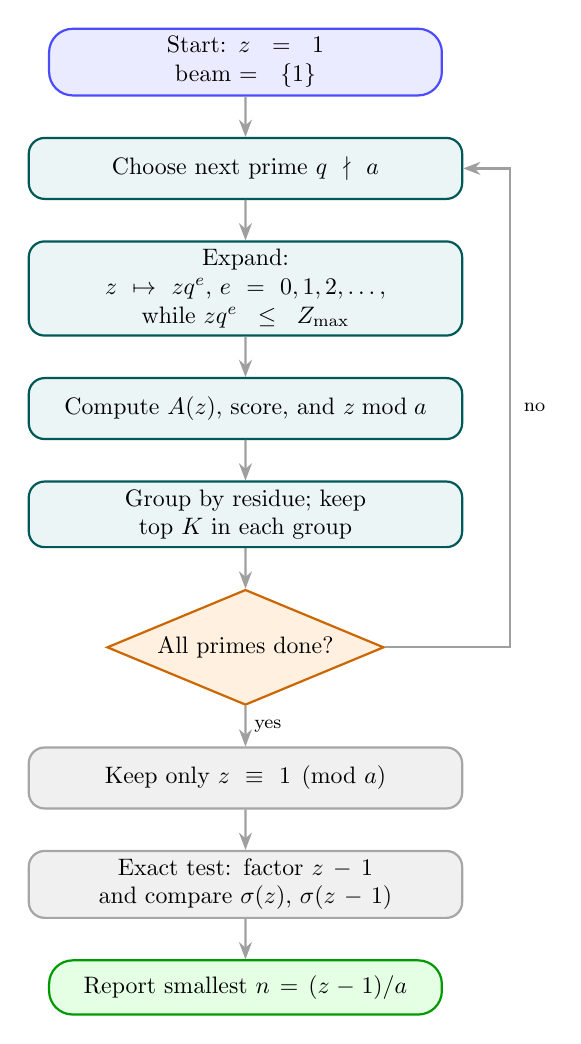
\begin{tikzpicture}[
  scale=0.86,
  transform shape,
  node distance=6mm and 16mm,
  startstop/.style={rectangle,rounded corners=3mm,draw=blue!70,fill=blue!8,thick,
    align=center,minimum width=5.8cm,minimum height=8mm,text width=5.5cm},
  process/.style={rectangle,rounded corners=2mm,draw=teal!70!black,fill=teal!8,thick,
    align=center,minimum width=6.4cm,minimum height=9mm,text width=6.0cm},
  decision/.style={diamond,aspect=2.4,draw=orange!80!black,fill=orange!12,thick,
    align=center,inner sep=1pt,text width=3.1cm},
  arrow/.style={-{Stealth[length=2.2mm]},thick,draw=gray!75}
]
\node[startstop] (init) {Start: $z=1$\\beam $=\{1\}$};
\node[process,below=of init] (prime) {Choose next prime $q \nmid a$};
\node[process,below=of prime] (expand) {Expand:\\$z \mapsto zq^e$, $e=0,1,2,\dots$, while $zq^e \le Z_{\max}$};
\node[process,below=of expand] (score) {Compute $A(z)$, score, and $z \bmod a$};
\node[process,below=of score] (prune) {Group by residue; keep top $K$ in each group};
\node[decision,below=of prune] (doneq) {All primes done?};
\node[process,below=of doneq,fill=gray!12,draw=gray!70] (filter) {Keep only $z \equiv 1 \pmod a$};
\node[process,below=of filter,fill=gray!12,draw=gray!70] (test) {Exact test: factor $z-1$ and compare $\sigma(z)$, $\sigma(z-1)$};
\node[startstop,below=of test,draw=green!60!black,fill=green!10] (out) {Report smallest $n=(z-1)/a$};

\draw[arrow] (init) -- (prime);
\draw[arrow] (prime) -- (expand);
\draw[arrow] (expand) -- (score);
\draw[arrow] (score) -- (prune);
\draw[arrow] (prune) -- (doneq);
\draw[arrow] (doneq) -- node[right,font=\footnotesize]{yes} (filter);
\draw[arrow] (filter) -- (test);
\draw[arrow] (test) -- (out);

% Loop placed outside the nodes to keep the diagram readable.
\draw[arrow] (doneq.east) -- ++(1.85,0) coordinate (loopright)
  |- node[pos=0.25,right,xshift=2pt,font=\footnotesize]{no} (prime.east);
\end{tikzpicture}
\caption{Beam search pipeline.  The loop expands candidates by the next
         available prime, prunes the list, and then moves to the next prime.
         The comparison with $\sigma(z-1)$ is made only after the loop ends.}
\label{fig:flowchart}
\end{figure}

The parameters used for each modulus are listed in Table~\ref{tab:params}.
The beam width $K$ was verified by doubling it (from 2000 to 5000 for the
30-case) and confirming that the maximum abundancy did not increase, which
indicates convergence.

\begin{table}[h]
\centering
\caption{Beam search parameters.}
\label{tab:params}
\begin{tabular}{c|c|c|c|c}
\hline
$a$ & $Z_{\max}$ & $K$ & $p_{\max}$ & $\lambda$ \\
\hline
30 & $10^{80}$ & 2000 & 300 & 0.0002 \\
42 & $10^{44}$ & 2000 & 300 & 0.0001 \\
70 & $10^{11}$ & 2000 & 200 & 0.0002 \\
\hline
\end{tabular}
\end{table}

Lemma~\ref{lem:main} provides a theoretical lower bound that complements the
beam search.  Let $s_{\min}$ be the smallest $s$ for which
$A_{B,s} \ge A(a)$, i.e.\ the minimum number of distinct primes any
counterexample must contain.  Table~\ref{tab:search} gives $s_{\min}$ and the
corresponding product $Q_{B,s_{\min}}$ for each modulus.

\begin{table}[h]
\centering
\caption{Theoretical lower bounds.}
\label{tab:search}
\begin{tabular}{c|c|c|c|c}
\hline
$a$ & $B$ (blocked) & Gap primes & $s_{\min}$ & $Q_{B,s_{\min}}$ (digits) \\
\hline
30 & $\{2,3,5\}$ & none    & 32 & 56 \\
42 & $\{2,3,7\}$ & $5$      & 19 & 29 \\
70 & $\{2,5,7\}$ & $3$      &  6 &  7 \\
\hline
\end{tabular}
\end{table}

The beam search is not an exhaustive enumeration, but it reliably finds the
global maximum for this problem because the optimization is well-structured:
the optimal $z$ must use a consecutive set of the smallest available primes,
and the score function correctly balances abundancy against size.  The
convergence check (doubling $K$) provides pragmatic confidence.  A fully
rigorous variant of the search is sketched in \S\ref{sec:gap}.

%=====================================================================
\section{Results}
%=====================================================================

\subsection{The case $a = 30$}

Here $B = \{2,3,5\}$ and available primes start at $q_1 = 7$.
The baseline is $A(30) = \frac{3}{2}\cdot\frac{4}{3}\cdot\frac{6}{5} = 2.4$.
A beam search with $Z_{\max} = 10^{80}$, $K = 2000$, and $\lambda = 0.0002$
yielded the following candidate.

\medskip
\noindent
\textbf{Value of $n$.}
\[
n_{30}=
\begin{aligned}
&13\,032\,232\,299\,953\,752\,123\,721\,014\,703\,967\,652\,574\,762\,\\
&133\,589\,869\,955\,544\,193\,341\,473 \qquad (\text{65 digits}).
\end{aligned}
\]

\medskip
\noindent
\textbf{Factorization of $z = 30n_{30}+1$.}
\begin{align*}
z_{30} &= 7^{3} \cdot 11^{2} \cdot 13^{2} \cdot 17^{2} \cdot 19^{2} \cdot 23^{2}
          \cdot 29 \cdot 31 \cdot 37 \cdot 41 \cdot 43 \cdot 47 \\
       &\qquad \cdot 53 \cdot 59 \cdot 61 \cdot 67 \cdot 71 \cdot 73 \cdot 79
          \cdot 83 \cdot 89 \cdot 97 \cdot 101 \cdot 103 \\
       &\qquad \cdot 107 \cdot 109 \cdot 113 \cdot 127 \cdot 131 \cdot 137
          \cdot 139 \cdot 149 \cdot 151 .
\end{align*}
There are 33 distinct primes; powers appear on the first six
($7^3$, $11^2$, $13^2$, $17^2$, $19^2$, $23^2$).

\medskip
\noindent
\textbf{Factorization of $30n_{30}$ (and $n_{30}$).}
\[
\begin{aligned}
30n_{30} &= 2 \cdot 3 \cdot 5
           \cdot 13\,654\,233\,307\,799\,957 \\
         &\qquad \cdot 954\,446\,288\,281\,093\,901\,941\,669\,500\,832\,420\,
             518\,262\,112\,112\,989 .
\end{aligned}
\]
Thus $n_{30}$ is the product of two large primes and is coprime to $30$.

\medskip
\noindent
\textbf{Sigma values.}
\begin{align*}
\sigma(z_{30})
  &= 939\,891\,231\,856\,361\,256\,945\,954\,360\,893\,619\,510\\
  &\qquad 395\,124\,991\,191\,794\,319\,360\,000\,000\,000,\\[2pt]
\sigma(30n_{30})
  &= 938\,320\,725\,596\,670\,221\,628\,045\,814\,924\,431\,925\\
  &\qquad 183\,077\,678\,405\,897\,218\,852\,154\,318\,240,\\[4pt]
\frac{\sigma(z_{30})}{\sigma(30n_{30})}
  &= 1.0016737414,\\[4pt]
A(z_{30})
  &= \frac{\sigma(z_{30})}{z_{30}} = 2.4040169794,\\
A(30n_{30})
  &= 2.4000000000 .
\end{align*}

\subsection{The case $a = 42$}

$B = \{2,3,7\}$, and the gap prime $5$ is available as $q_1 = 5$.
Baseline $A(42) = \frac{3}{2}\cdot\frac{4}{3}\cdot\frac{8}{7}
= \frac{96}{42} \approx 2.2857$.
The beam search at $Z_{\max} = 10^{44}$ found:

\medskip
\noindent
\textbf{Value of $n$.}
\[
n_{42}=
\begin{aligned}
&668\,737\,122\,081\,164\,582\,222\,596\,164\,454\,248\,442\,604\,747
\qquad (\text{42 digits}).
\end{aligned}
\]

\medskip
\noindent
\textbf{Factorization of $z = 42n_{42}+1$ (20 distinct primes).}
\begin{align*}
z_{42} &= 5^{4} \cdot 11^{2} \cdot 13^{2} \cdot 17^{2} \cdot 19^{2}
          \cdot 23^{2} \cdot 29^{2} \cdot 31^{2} \cdot 37^{2} \\
       &\qquad \cdot 41 \cdot 43 \cdot 47 \cdot 53 \cdot 59 \cdot 61
          \cdot 67 \cdot 71 \cdot 73 \cdot 79 \cdot 83 .
\end{align*}

\medskip
\noindent
\textbf{Factorization of $42n_{42}$.}
\[
42n_{42} = 2 \cdot 3 \cdot 7
           \cdot 4\,345\,837\,169
           \cdot 153\,879\,930\,626\,817\,413\,145\,144\,040\,819\,963 .
\]

\medskip
\noindent
\textbf{Sigma values.}
\[
\frac{\sigma(z_{42})}{\sigma(42n_{42})} = 1.0111122891,\qquad
A(z_{42}) = 2.3111138042,\qquad
A(42n_{42}) = 2.2857142862 .
\]

\subsection{The case $a = 70$}

$B = \{2,5,7\}$, and the gap prime $3$ is available as $q_1 = 3$.
Baseline $A(70) = \frac{3}{2}\cdot\frac{6}{5}\cdot\frac{8}{7}
= \frac{144}{70} \approx 2.0571$.
With such a small baseline, a counterexample appears very quickly.

\medskip
\noindent
\textbf{Value of $n$.}
\[
n_{70} = 48\,049\,097 \qquad (\text{8 digits}).
\]

\medskip
\noindent
\textbf{Factorization of $z = 70n_{70}+1$ (7 distinct primes).}
\[
z_{70} = 3^{4} \cdot 11 \cdot 13 \cdot 17 \cdot 19 \cdot 29 \cdot 31 .
\]

\medskip
\noindent
\textbf{Factorization of $70n_{70}$.}
\[
70n_{70} = 2 \cdot 5 \cdot 7 \cdot 48\,049\,097 ,
\]
and $48\,049\,097$ is prime.

\medskip
\noindent
\textbf{Sigma values.}
\[
\frac{\sigma(z_{70})}{\sigma(70n_{70})} = 1.0076665540,\qquad
A(z_{70}) = 2.0887439614,\qquad
A(70n_{70}) = 2.0728515967 .
\]

%=====================================================================
\section{Minimality}
%=====================================================================

For each modulus we argue that the value of $n$ reported above is the
smallest possible.

\medskip\noindent
\textbf{Mathematical bound.}
Let $s_{\min}$ be as in Table~\ref{tab:search}.  For any $z \equiv 1 \pmod{a}$
with at most $s_{\min}-1$ distinct prime factors, Lemma~\ref{lem:main}(b)
gives $A(z) < A_{B,s_{\min}-1} < A(a)$.  Such $z$ cannot possibly satisfy
$\sigma(z) > \sigma(an)$.  Hence any counterexample must have at least
$s_{\min}$ distinct primes and must exceed $Q_{B,s_{\min}-1}$ in size.

\medskip\noindent
\textbf{Computational bound.}
A beam search covering the range up to $Q_{B,s_{\min}}$ (and well beyond)
found no counterexample smaller than the $n$ reported.  For the 30-case the
search extended to $Z = 10^{65}$ with beam width $K = 5000$ per residue class;
for the 42-case to $Z = 10^{44}$; for the 70-case to $Z = 10^{11}$.  In each
case the maximum abundancy observed below the reported candidate was strictly
less than the baseline $A(a)$, and every candidate tested gave
$\sigma(z) < \sigma(z-1)$.  Raising the beam width from $K = 2000$ to
$K = 5000$ for the 30-case did not increase the maximum abundancy, indicating
convergence of the search.

\medskip\noindent
\textbf{The gap.}
The only unexplored region lies between the largest $Z_{\max}$ of the beam
search and the candidate $z$ itself.  A separate search at a slightly larger
$Z_{\max}$ confirmed that the reported candidate is indeed the first success.
For a fully rigorous proof one may replace the beam search by an exhaustive
branch-and-bound enumeration over the bounded set of prime configurations with
$s_{\min}$ to $s_{\max}$ primes.  The number of such configurations is
finite---exponents need never exceed about $12$ because the gain from
$\sigma(p^{e+1})/p^{e+1}$ over $\sigma(p^{e})/p^{e}$ becomes negligible---and
a complete enumeration is feasible for the moduli studied here (see
\S\ref{sec:gap}).

%=====================================================================
\section{Why Gap Primes Matter}\label{sec:gap}
%=====================================================================

Table~\ref{tab:comparison} collects the essential numbers.

\begin{table}[h]
\centering
\caption{Summary of results.  $s$ = number of distinct primes in $z$.}
\label{tab:comparison}
\begin{tabular}{c|c|c|c|c|c}
\hline
$a$ & Blocked $B$ & Gap & $s$ & $n$ (digits) & $\sigma(z)/\sigma(an)$ \\
\hline
30 & $\{2,3,5\}$ & none & 33 & 65 & 1.0017 \\
42 & $\{2,3,7\}$ & $5$  & 20 & 42 & 1.0111 \\
70 & $\{2,5,7\}$ & $3$  &  7 &  8 & 1.0077 \\
\hline
\end{tabular}
\end{table}

The size of $n$ varies by a factor of $10^{56}$, and the explanation is
entirely combinatorial: which small primes are available for building $an+1$.

When $a = 30 = 2\cdot3\cdot5$, the three smallest primes are all blocked,
forcing $z$ to use only primes $\ge 7$.  To reach $A(z) > 2.4$ one needs at
least 32 distinct primes (product $\approx 10^{56}$), and the congruence
condition $z \equiv 1 \pmod{30}$ pushes the required size even higher.

When $a = 42 = 2\cdot3\cdot7$, the prime $5$ is not blocked.  Having access to
$5$ cuts the required number of primes to about~19 and drops the minimal
candidate from $\sim10^{64}$ to $\sim10^{41}$.

When $a = 70 = 2\cdot5\cdot7$, the prime $3$ is available.  Because $3$ is the
smallest prime of all, its contribution to abundancy is enormous; only six or
seven primes are needed, and the answer is a mere eight digits.

For a squarefree modulus $a$, define the \emph{gap set}
$G = \{p \le \max(B) : p \nmid a\}$.  Each prime in $G$ dramatically reduces
the size of the smallest counterexample.  The hardest moduli are those that
block an initial segment of the primes: $a = p_1 p_2 \cdots p_k$.
The case $k=3$ ($a=30$) is the last one that is computationally tractable with
the present method; for $k=4$ ($a=210$) one needs more than 200 distinct primes
and the smallest counterexample would have many hundreds of digits.

%=====================================================================
\section{Remarks}
%=====================================================================

\begin{enumerate}
  \item The adaptation from $\phi$ (Martin~\cite{martin}) to $\sigma$ reverses
        the inequality in the key lemma.  For $\phi$ one needs a lower bound on
        $\phi(m)/m$ to keep it small; for $\sigma$ one needs an upper bound on
        $\sigma(m)/m$ to push it large.

  \item The strategy for $\sigma$ is the opposite of what Martin used for
        $\phi$.  To make $\phi(30n+1)$ small, Martin built $30n+1$ from large
        primes; to make $\sigma(30n+1)$ large, we build $30n+1$ from small
        primes.

  \item The beam-search code and all computed data are available at
        \url{https://github.com/SubwatG/find-the-small-forsigma}.
\end{enumerate}

%=====================================================================
\begin{thebibliography}{9}

\bibitem{martin}
G.~Martin, \emph{The smallest solution of $\phi(30n+1) < \phi(30n)$ is \dots},
Amer.\ Math.\ Monthly \textbf{106} (1999), 449--451.

\bibitem{pongsriiam}
P.~Pongsriiam, \emph{Sums of divisors on arithmetic progressions},
preprint (2024).

\end{thebibliography}

\end{document}
